\documentclass[pdflatex,compress,mathserif]{beamer}

%\usetheme[dark,framenumber,totalframenumber]{ElektroITK}
\usetheme[darktitle,framenumber,totalframenumber]{ElektroITK}

\usepackage[utf8]{inputenc}
\usepackage[T1]{fontenc}
\usepackage{lmodern}
\usepackage[bahasai]{babel}
\usepackage{amsmath}
\usepackage{amsfonts}
\usepackage{amssymb}
\usepackage{graphicx}
\usepackage{multicol}
\usepackage{lipsum}

\newcommand*{\Scale}[2][4]{\scalebox{#1}{$#2$}}%

\title{Sinyal dan Sistem}
\subtitle{Sinyal dan Sistem}

\author{Tim Dosen Pengampu}

\begin{document}

\maketitle

\section{Sinyal Waktu Kontinyu dan Sinyal Waktu Diskrit}

\begin{frame}
	\frametitle{Sinyal}
	\begin{center}
		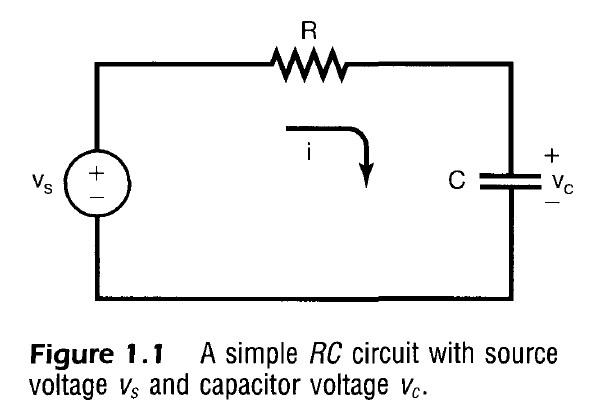
\includegraphics[width=0.7\linewidth]{img/img01}
	\end{center}
\end{frame}

\begin{frame}{Sinyal}
	\begin{center}
		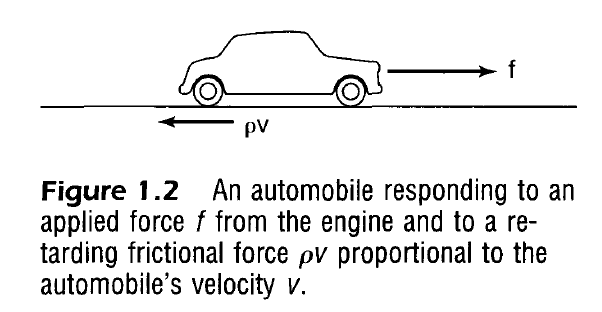
\includegraphics[width=0.7\linewidth]{img/img02}
	\end{center}
\end{frame}

\begin{frame}{Sinyal}
	\begin{center}
		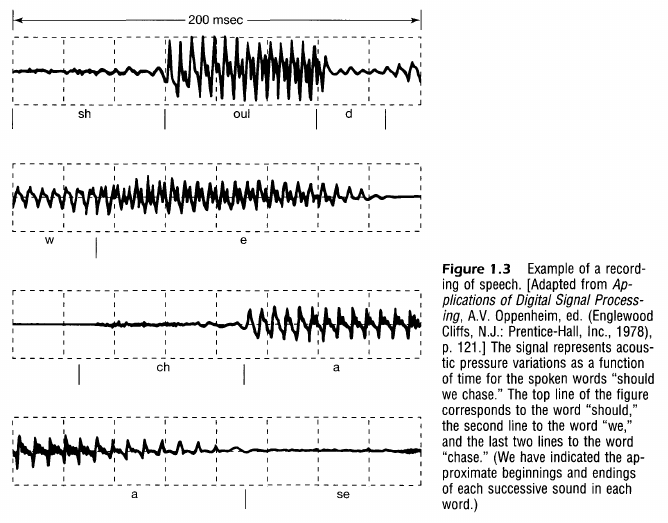
\includegraphics[width=0.7\linewidth]{img/img03}
	\end{center}
\end{frame}

\begin{frame}{Sinyal}
	\begin{center}
		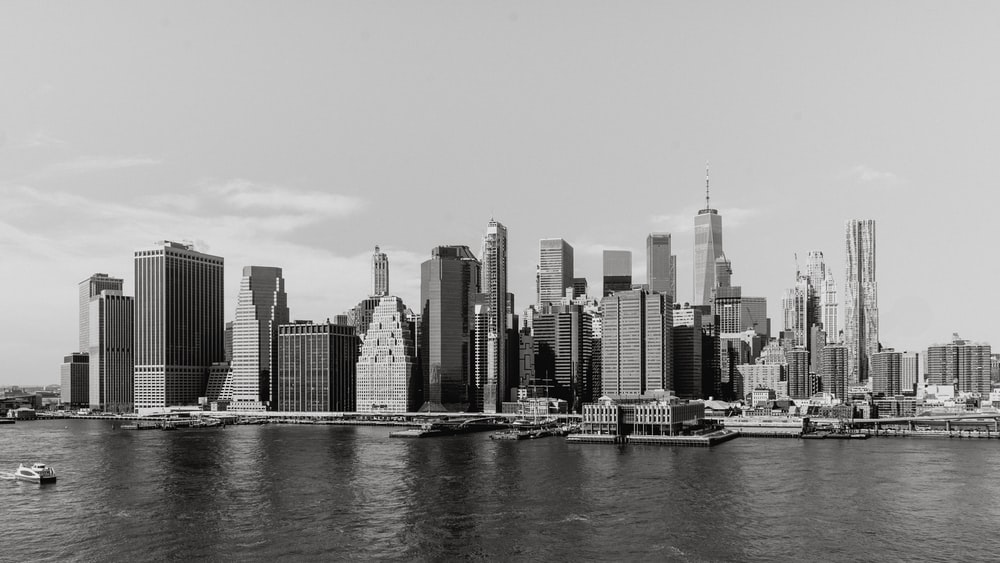
\includegraphics[width=0.7\linewidth]{img/img04}
	\end{center}
\end{frame}

\begin{frame}{Sinyal}
	\begin{center}
		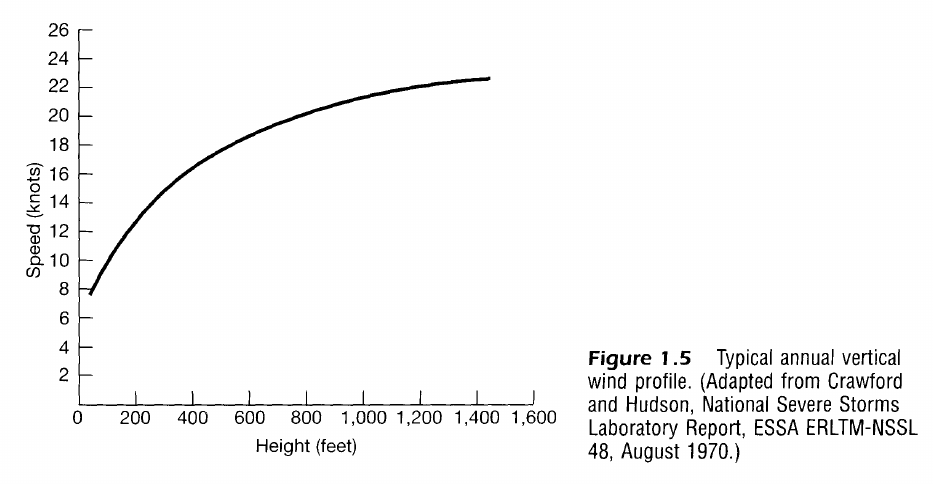
\includegraphics[width=0.7\linewidth]{img/img05}
	\end{center}
\end{frame}

\begin{frame}{Sinyal}
	\begin{enumerate}
		\item Sinyal waktu kontinyu
		\item Sinyal waktu diskrit
	\end{enumerate}
\end{frame}

\begin{frame}{Sinyal}
	\begin{center}
		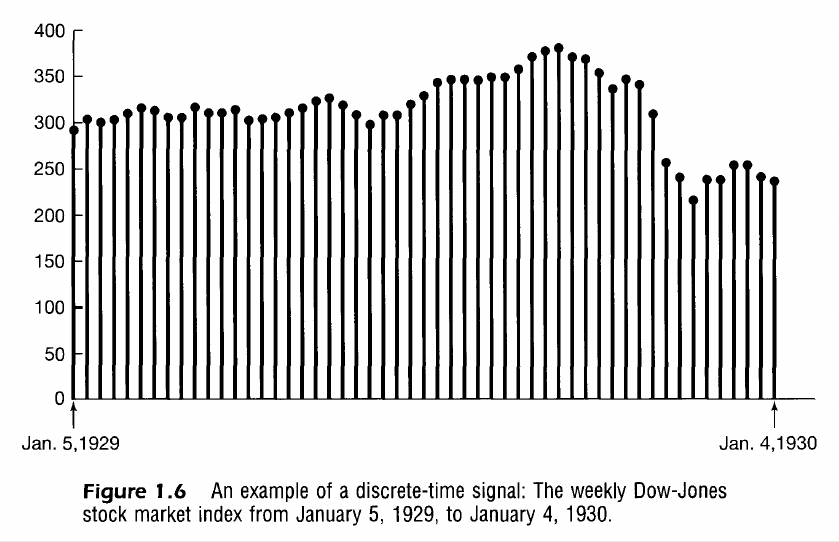
\includegraphics[width=0.7\linewidth]{img/img06}
	\end{center}
\end{frame}

\begin{frame}{Sinyal}
	\begin{enumerate}
		\item Notasi sinyal waktu kontinyu x(t)
		\item Notasi sinyal waktu diskrit x[n]
	\end{enumerate}
\end{frame}

\begin{frame}{Sinyal}
	\begin{center}
		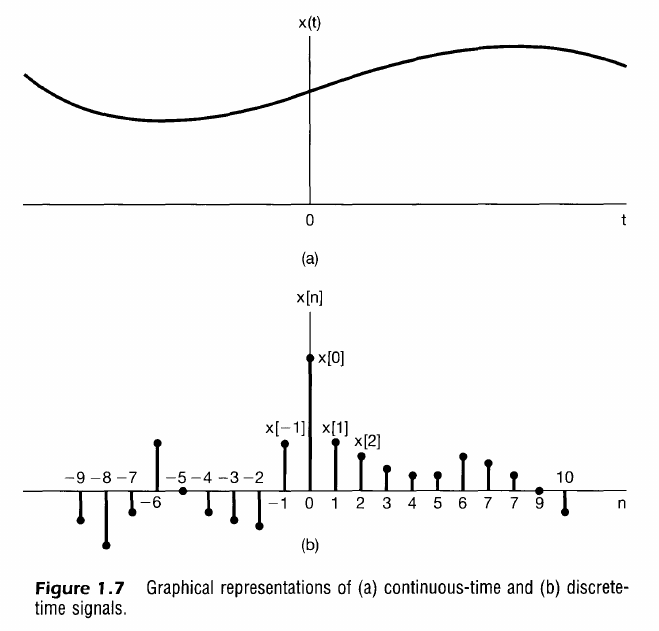
\includegraphics[width=0.7\linewidth]{img/img07}
	\end{center}
\end{frame}

\begin{frame}
	\frametitle{Daya dan Energi Sinyal}
	\begin{multicols}{2}
		\begin{center}
			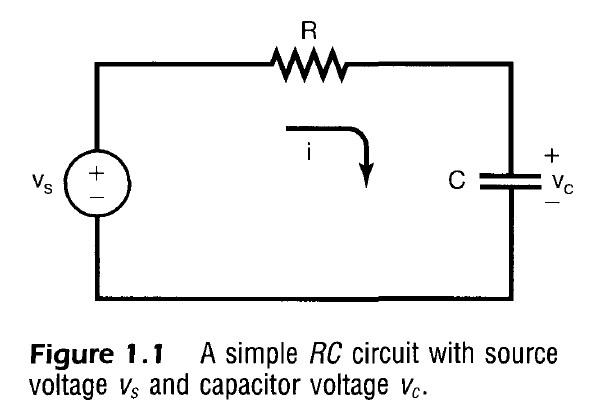
\includegraphics[width=\linewidth]{img/img01}
		\end{center}
		\columnbreak
		Daya:\\
		\begin{center}
			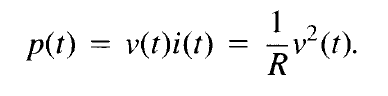
\includegraphics[width=0.7\linewidth]{img/img08}
		\end{center}
		Energi total:\\
		\begin{center}
			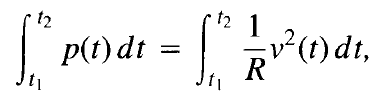
\includegraphics[width=0.7\linewidth]{img/img09}
		\end{center}
		Daya rata-rata:\\
		\begin{center}
			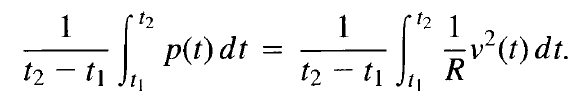
\includegraphics[width=\linewidth]{img/img10}
		\end{center}
	\end{multicols}
\end{frame}

\begin{frame}{Daya dan Energi Sinyal}
	\begin{multicols}{2}
		\begin{center}
			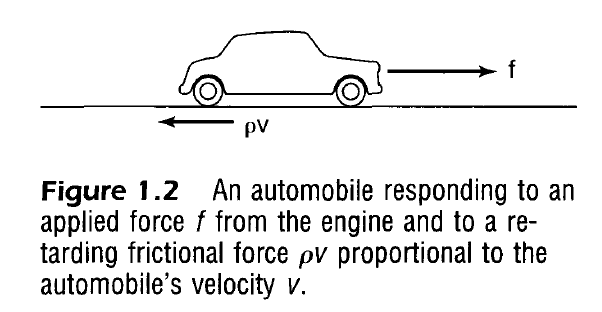
\includegraphics[width=\linewidth]{img/img02}
		\end{center}
		\columnbreak
		Daya:\\
		\begin{center}
			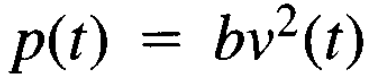
\includegraphics[width=0.5\linewidth]{img/img11}
		\end{center}
		Energi total: ? \\
		Daya rata-rata: ?\\
	\end{multicols}
\end{frame}

\begin{frame}{Daya dan Energi Sinyal}
	\begin{itemize}
		\item Energi total dalam interval $ t_1 \leq t \leq t_2 $ dalam sinyal waktu kontinyu $ x(t) $
		\begin{center}
			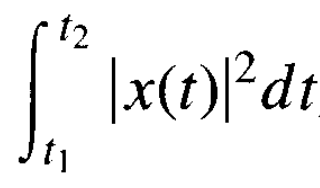
\includegraphics[width=0.2\linewidth]{img/img12}
		\end{center}
		$ |x(t)| $ adalah magnitude dari $ x $
		
		\item Energi total dalam interval $ n_1 \leq n \leq n_2 $ dalam sinyal waktu diskrit $ x[n] $
		\begin{center}
			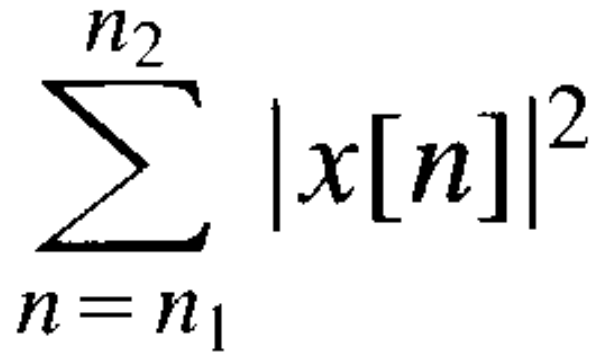
\includegraphics[width=0.2\linewidth]{img/img13}
		\end{center}
		$ |x(n)| $ adalah magnitude dari $ x $
	\end{itemize}
\end{frame}

\begin{frame}{Daya dan Energi Sinyal}
	\begin{itemize}
		\item Energi total dalam interval $ -\infty \leq t \leq \infty $ dalam sinyal waktu kontinyu $ x(t) $
		\begin{center}
			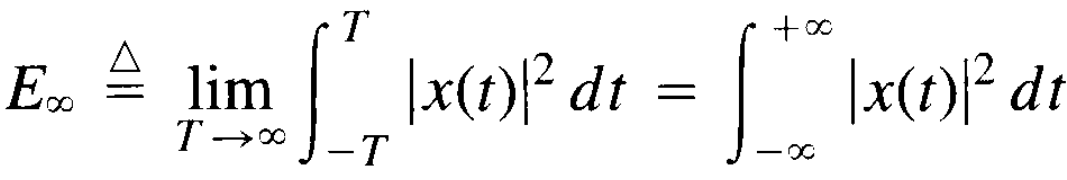
\includegraphics[width=0.5\linewidth]{img/img14}
		\end{center}
		
		\item Energi total dalam interval $ -\infty \leq n \leq \infty $ dalam sinyal waktu diskrit $ x[n] $
		\begin{center}
			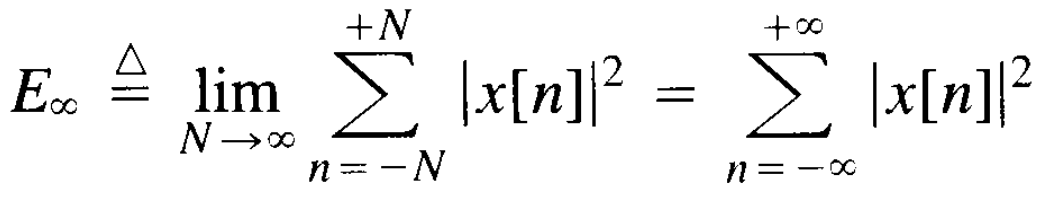
\includegraphics[width=0.5\linewidth]{img/img15}
		\end{center}
		
		\item Kedua persamaan di atas bisa saja tidak konvergen.
		\item Jika $ x(t) $ dan $ x[n] $ sama dengan konstanta bukan nol di semua $ t $, maka sinyal tersebut memiliki energi yang tak hingga.
	\end{itemize}
\end{frame}

\begin{frame}{Daya dan Energi Sinyal}
	\begin{itemize}
		\item Daya rata-rata dalam interval $ -\infty \leq t \leq \infty $ dalam sinyal waktu kontinyu $ x(t) $
		dan sinyal waktu diskrit $ x[n] $
		\begin{center}
			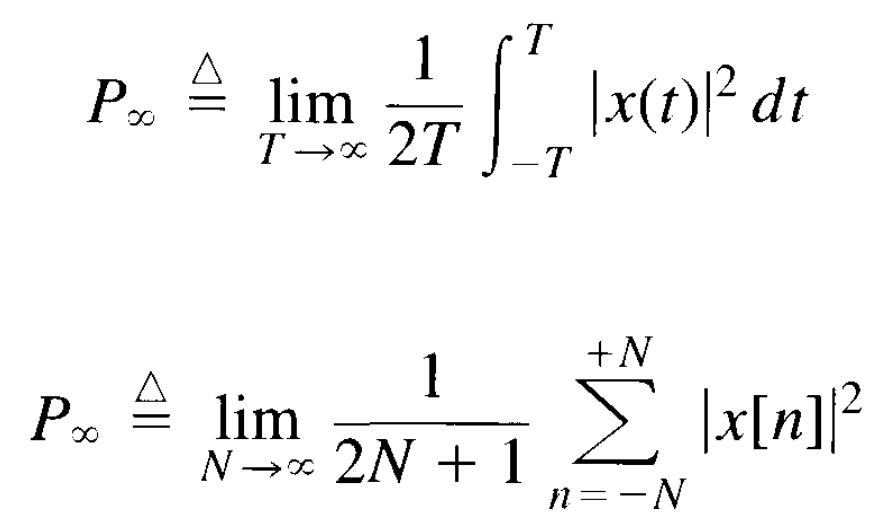
\includegraphics[width=0.5\linewidth]{img/img16}
		\end{center}
		
	\end{itemize}
\end{frame}

\section{Sinyal Eksponensial dan Sinyal Sinusoidal}

\section{Fungsi Unit Impulse dan Fungsi Unit Step}

\section{Sistem Waktu Kontinyu dan Sistem Waktu Diskrit}

\section{Sifat-Sifat Dasar Sistem}


\end{document}
